\documentclass[tikz,border=10pt]{standalone}
\usepackage{tikz}
\usetikzlibrary{decorations.pathmorphing}

\begin{document}

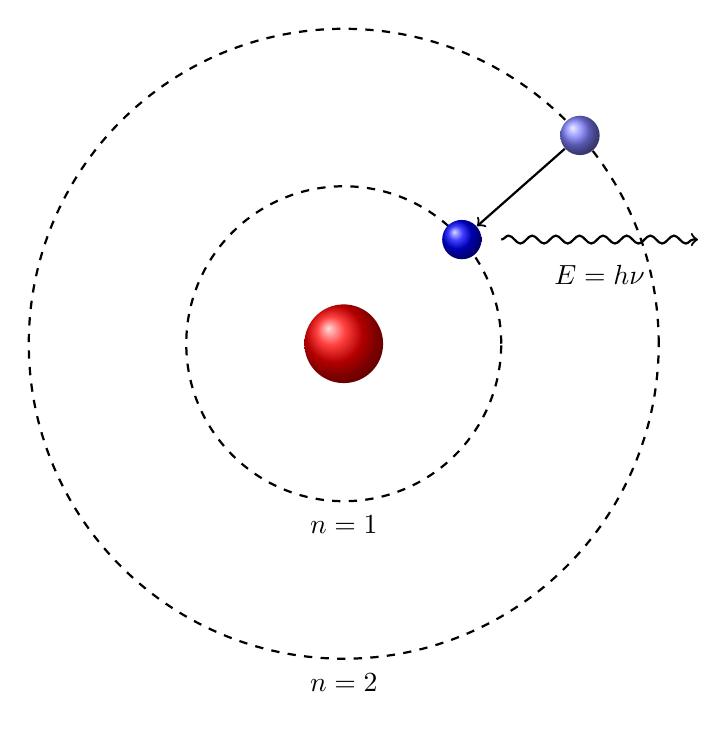
\begin{tikzpicture}

  % Nucleus
  \node[ball color=red, circle, minimum size=1cm] (nucleus) at (0,0) {};

  % Energy levels
  \draw[thick,dashed] (0,0) circle (2cm);
  \node at (0,-2.3) {\textbf{\(n = 1\)}};

  \draw[thick,dashed] (0,0) circle (4cm);
  \node at (0,-4.3) {\textbf{\(n = 2\)}};

  % Electrons
  \node[ball color=blue!50, circle, minimum size=0.5cm] (electron_outer) at (3,{sqrt(7)}) {};
  \node[ball color=blue, circle, minimum size=0.5cm] (electron_inner) at (1.5,{sqrt(1.75)}) {};

  % Electron transition
  \draw[->, thick] (electron_outer) -- (electron_inner);

  % Photon emission (wavy arrow)
  \draw[->, thick, decorate, decoration={snake, amplitude=0.5mm, segment length=3mm}] 
    (electron_inner) + (0.5,0) -- +(3,0) node[midway, below=0.2cm] {\( E = h\nu\)};

\end{tikzpicture}

\end{document}
